\documentclass[reqno]{amsart}

\usepackage{External/takodachi}

% To show labels in the margin:
\usepackage[notref, notcite]{showkeys}

\usepackage{slashed}

\newcommand{\II}{\mathrm{II}}	% Second fundamental form
\newcommand{\sfED}{\mathsf{ED}}

\title
{
	Large-data theory for wave maps on $\R^{1 + 2}$
} 
\author{Jason Zhao}
\date{\today}


\begin{document}
\maketitle

\begin{abstract}
	In these notes we present the large-data theory for the energy-critical wave maps equation a l\'a the \textit{energy dispersion method} of Sterbenz and Tataru in their series of papers	\cite{SterbenzTataru2010, SterbenzTataru2010a}. 
\end{abstract}

\tableofcontents

\section{Introduction}
Before getting into any multi-linear algebra, it is important to get a grasp of coordinates in linear algebra and how these coordinates respond to change of bases. Let $V$ be an $n$-dimensional real vector space, and denote $V^*$ its dual space. Given a basis $\{e_i\}_i \subseteq V$, there exists a dual basis $\{\epsilon^j\}_j \subseteq V^*$ satisfying 
	\[ \langle e_i, \epsilon^j \rangle = \delta^j_i. \]
Choose another basis $\{\widetilde e_i\}_i \subseteq V$ and denote its dual basis by $\{\widetilde \epsilon^j\}_j \subseteq V^*$. There exists a change of basis matrix $C^k_i \in \mathsf{GL} (\R^n)$ sending the original basis to the new basis,
	\[ \widetilde e_i = C^k_i e_k. \]	
On the other hand, the inverse change of basis matrix $(C^{-1})^j_k \in \mathsf{GL} (\R^n)$, i.e. $(C^{-1})^j_k C^k_i = \delta^j_i$, transforms the original dual basis to the new dual basis 	
	\[ \widetilde \epsilon^j = (C^{-1})^j_k \epsilon^k. \]
Throughout these notes, we will use these \emph{Einstein summation notation}, where repeated indices are summed over, e.g. $a^i b_i := \sum_i a^i b_i$.


\subsection{{Contravariance}}

We say an object is \emph{contravariant} if the coordinate representation \textit{contra-varies} with respect to change of basis, that is, transforms by the inverse matrix $(C^{-1})^j_i$. Such coordinates are indexed by \textit{upper indices}. The prototypical example of a contravariant object is a \emph{vector} $v \in V$. Every vector admits a unique coordinate representation $\{v^i\}_i \subseteq \R$ with respect to the basis $\{e_i\}_i$, i.e.
	\[ v = v^i e_i . \]
Let $\{ \widetilde v^j \}_j \subseteq \R$ be the unique coordinates with respect to the basis $\{\widetilde e_j\}_j$, then the change of coordinates from $\{v^i\}_i$ to $\{\widetilde v^j\}_j$ is given by the inverse change of basis matrix,
	\[ \widetilde v^j = {(C^{-1})}^j_i v^i. \]
Indeed, 	
	\[ v = \widetilde v^j \widetilde e_j  = \left( {(C^{-1})}^j_i v^i \right) \left( C^k_j e_k \right) = \delta^k_i v^i e_k = v^i e_i . \]
We can interpret a choice of basis $\{e_i\}_i$ as endowing $V$ with a ``measuring tool'', where the coordinates $\{v^i\}_i$ representing the resulting ``measurement''. A change of basis corresponds to changing the choice of ``measuring tool'', e.g. we can view a change of basis $\widetilde e_i = \tfrac{1}{100} e_i$ as changing from ``meters'' $e_i$ to ``centimeters'' $\widetilde e_i$, so the corresponding change of coordinates is 
	\[ \widetilde v^i \text{ meters } = 100 v^i \text{ centimeters}. \]




\subsection{Covariance}

We say that an object is \emph{covariant} if the coordinate representation \textit{co-varies} with respect to change of basis, that is, transforms by the matrix $C^k_i$.  Such coordinates are indexed by \textit{lower indices}. The prototypical example of a covariant object is a \emph{covector} $\omega \in V^*$. Every covector admits a unique coordinate representation $\{\omega_i \}_i \subseteq \R$ with respect to the basis $\{\epsilon^i\}_i$, i.e.
	\[ \omega = \omega_i \epsilon^i = \widetilde \omega_j \widetilde \epsilon^j. \]
Let $\{\widetilde \omega_j \}_j \subseteq \R$ be the unique coordinates with respect to the basis $\{\widetilde \epsilon^j\}_j$, then the change of coordinates from $\{\omega_i\}_i$ to $\{\widetilde \omega_j\}_j$ is given by the change of basis matrix,
	\[ \widetilde \omega_j = C^i_j \omega_i \]
Indeed, 
	\[ \omega = \widetilde \omega_j \widetilde \epsilon^j = \left( C^i_j \omega_i \right) \left( (C^{-1})_k^j \epsilon^k \right) =  \delta^i_k \omega_i \epsilon^k = \omega_i \epsilon^i. \]
Scalars are regarded as ``dimensionless'' quantities, so since a covector acting on a vector produces a scalar, they have inverse dimensions. For example, we can view a change of basis $\widetilde \epsilon^j = 100 \epsilon^j$ as changing from  ``meters$^{-1}$'' $\epsilon^j$ to ``centimeters$^{-1}$'' $\widetilde \epsilon^j$, so the corresponding change of coordinates is 
	\[ \widetilde \omega_j \text{ meters$^{-1}$} = \frac{1}{100} \omega_j  \text{ centimeters$^{-1}$}. \]



\section{Energy dispersion method}



Energy dispersion
	\[ \sfED [\phi] = \sup_{N \in 2^\Z} ||P_N \phi||_{L^\infty_{t, x} [I]} \]
Scaling dictates that 
	\[ ||P_N \phi||_{L^\infty_x} \lesssim ||\phi||_{\dot H^1_x} \]	
So while we do not have the endpoint embedding $\dot H^1 \subseteq L^\infty$, we do have this embedding into the energy dispersion space.

\begin{theorem}[Energy-dispersed regularity theorem]
	There exist functions $F(\cE) \gg 1$ and $\epsilon (\cE) \ll 1$ of energy such that if $\phi : [t_0, t_1] \times \R^2 \to \MM$ is a solution to the wave maps equation \eqref{wave} with finite energy $\cE[\phi] \equiv \cE$ and energy dispersion
		\begin{equation}
			||\phi||_{\sfED [I]} \leq \epsilon (\cE), 
		\label{eq:ED}
		\end{equation}
	then 
		\begin{equation}
			||\phi||_{\sfS [I]} \leq \cF(\cE).
		\label{eq:S}
		\end{equation}
	In addition, there exists a polynomial $K(\cF)$ such that if $\{c_\kappa\}_\kappa$ is any $(\delta_0, \delta_1)$-admissible frequency envelope for $\vec \phi_0$, we have the bound 
		\[ ||\phi||_{\sfS_c [I]} \leq K(\cF(E)).  \]
	In particular, one may extend $\phi$ to a finite energy wave-map on the interval $(t_0 - T, t_1 + T)$ for some $T \ll_{\cE, c, \epsilon} 1$. \label{thm:ED}
\end{theorem}

\subsection{Induction on energy}

To illustrate the induction on energy scheme, we will aim for a qualitative statement, though as we detail the proof we will arrive at the full quantitative energy-dispersion theorem. We say that an energy $\cE$ is \emph{regular} if there exists parameters $\epsilon \ll 1$ sufficiently small and $\cF \gg 1$ sufficiently large such that for every wave map $\phi : I \times \R^2 \to \MM$ with energy $\cE [\phi] = \cE$ we have
	\[ ||\phi||_{\sfED [I]} \leq \epsilon \text{ implies } || \phi||_{\cS[I]} \leq \cF. \]
We remark that we are free to choose these parameters $\epsilon$ and $\cF$, though as we will soon see in the proof we can give a quantitative dependence on $\cE[\phi]$. Let us denote the set of regular energies by 
	\[ \cR := \{ \cE \in [0, \infty) : \text{$\cE$ is a regular energy} \}. \]
The global well-posedness theorem for small energy furnishes the base case for our induction on energy, $[0, \cE_0] \subseteq \cR$ for $\cE_0 \ll 1$ sufficiently small. Assume then for induction that energies are regular up to some $\cE_0$. Our goal is to construct a positive non-increasing function of energy $e (\cE) > 0$ to push the induction forward by showing that $\cE_0 + e$ is a regular energy for any $e \leq e (\cE_0)$. This induction step allows us to conclude the usual continuous induction argument, as it shows
	\begin{itemize}
		\item $\cR$ is open: if $[0, \cE_0] \subseteq \cR$ then $[0, \cE_0 + e(\cE_0)] \subseteq \cR$, 
		\item $\cR$ is closed: if we have a sequence of regular energies $\{ \cE_n \}_n \subseteq \cR$ such that $\cE_n \nearrow \cE$, then since $e :[0, \infty) \to (0, \infty)$ is positive non-increasing, $e(\cE_n) > e(\cE) > 0$. Taking $n$ large, we have $\cE \leq \cE_n + e(\cE_n)$ and therefore by the induction step $\cE$ is regular. 
	\end{itemize}
By connectedness, we conclude $\cR = [0, \infty)$, i.e. all energies are regular. 

\begin{remark}
	If instead $e(\cE_n) \to 0$ as $\cE_n \nearrow \cE$, e.g. if we were not precise and allowed $e$ to depend also on $\epsilon$ or $\cF$, then we would not be able to prove closedness of the set of regular energies. The Kenig-Merle strategy is to assume towards a contradiction that there exists a \emph{critical element}, i.e. a minimal energy blow-up solution, and then attempt to eliminate this possibility. 
	
	\begin{figure}[h]
		\begin{center}
			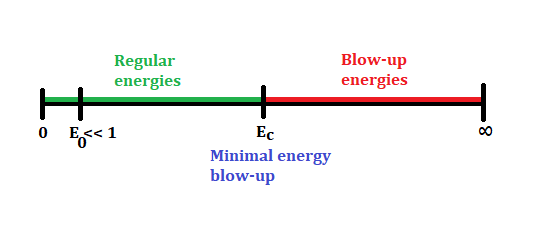
\includegraphics{graphics/kenigmerle}
			\caption{If the set of regular energies $\cR$ was not closed, i.e. $\cR = [0, \cE_c)$, then there would exist a minimal energy blow-up wave map $\cE [\phi_c] = \cE_c$. }
		\end{center}
	\end{figure}
\end{remark}

We end this subsection by getting the proof of the induction step started. Suppose for induction $\cE_0$ is a regular energy and $e \leq e(\cE_0) \ll 1$ a small energy increment to be chosen later. Let $\phi : I \times \R^2 \to \MM$ be a wave map with energy $\cE[\phi] = \cE_0 + e$ and energy dispersion 
	\[ ||\phi||_{\sfED[I]} \leq \epsilon.\]
We want to compare with a wave map $\widetilde \phi : I \times \R^2 \to \MM$ with an energy by hypothesis assumed to be regular $\cE[\widetilde \phi] = \cE_0$. Choose then a \emph{cut frequency} $k_* \in \R$ to truncate the initial data  such that its projection $\Pi$ back onto $T\mathbb M$ has regular energy,
	\[ \cE[\Pi P_{\leq k_*}  \phi[0]] = \cE_0. \]
Such a projection is well-defined since energy-dispersed solutions stay close to the manifold. Local well-posedness guarantees that there exists a solution $\widetilde \phi : J \times \R^2 \to \MM$ with initial data $\widetilde \phi[0] = \Pi P_{\leq k_*}  \phi[0]$ on some small time interval $J \subseteq I$. To make use of the fact $\cE_0$ is a regular energy, we need to pass the energy dispersion of $\phi$ to $\widetilde \phi$. The heuristic is that $\widetilde \phi[0] \approx P_{\leq k_*} \phi[0]$ up to higher-order errors. Indeed, 
	\begin{equation}
		||P_k (P_{\leq k_*} \phi [0] - \widetilde \phi[0]) ||_{\dot H^1 \times L^2} \lesssim_{\cE_0} \epsilon^{\frac14} 2^{-\frac12 |k - k_*|}.
	\end{equation}
The proof uses standard Moser-type estimates, i.e. chain rule and Bernstein's inequality, see \cite[Section 11]{SterbenzTataru2010}. The gain on the right-hand side allows us to use the Sobolev-Bernstein inequality to estimate the energy-dispersion of $\widetilde \phi$ at time $t = 0$ by 
	\begin{align*}
		||P_k \widetilde \phi [0]||_{L^\infty_x}
			&\leq ||P_k (P_{\leq k_*} \phi [0] - \widetilde \phi[0]) ||_{L^\infty_x} + ||P_k (P_{\leq k_*} \phi [0]||_{L^\infty_x} \\
			&\lesssim_{\cE_0} 2^{\frac{k}{2}} ||P_k (P_{\leq k_*} \phi [0] - \widetilde \phi[0]) ||_{\dot H^1 \times L^2}  + ||P_k \phi[0]||_{L^\infty_x}\lesssim_{k^*} \epsilon^{\frac14} + \epsilon \lesssim \epsilon^{\frac14}. 
	\end{align*}
Choosing then $\epsilon^{\frac14} \ll \epsilon (\cE_0)$, the local well-posedness theory guarantees that $\widetilde \phi$ is energy-dispersed in that, after possibly choosing a smaller time interval $J_0 \subseteq J \subseteq I$,  
	\[ ||\widetilde\phi||_{\sfED[J_0]} \leq \epsilon (\cE_0).  \]
Then the induction hypothesis guarantees that we have the dispersive bound
	\[ ||\widetilde \phi ||_{\sfS [J_0]} \leq \cF (\cE_0).  \]


\subsection{Bootstrap argument}


We want to propagate $\sfS$-control for the truncated solution $\widetilde\phi$ to our original solution $\phi$. We also want to propagate our estimates from the sub-interval $J \subseteq I$ to the full time interval $I$. To this end, suppose we have suitable choices of $e, \epsilon, \cF$, and let $\phi$ be a wave map such that 
	\begin{equation}
		||\phi||_{\sfED [I]} \leq \epsilon.
		\label{eq:ED1}
	\end{equation}
We make the following bootstrap assumptions on the sub-interval $J \subseteq I$,
	\begin{align}
		||\phi||_{\sfS [J]}
			&\leq 2 \cF , \label{eq:BS1}\\
		||\widetilde \phi||_{\sfED [J]}
			&\leq \widetilde \epsilon \label{eq:BS2},
	\end{align}
and aim to improve the bounds, 
	\begin{align}
		||\phi||_{\sfS [J]}
			&\leq \cF, \label{eq:BS1i} \\
		||\widetilde \phi||_{\sfED [J]}
			&\leq \frac12\widetilde\epsilon \label{eq:BS2i}. 		
	\end{align}
To conclude the proof of Theorem \ref{thm:ED} via a continuous induction on time, we need the following:


\begin{lemma}[Bootstrapping tool]
	Let $I$ be an interval and $\{ c_k \}_k$ a frequency envelope. Then for each affinely Schwartz function $\phi$ in $I$ the following properties hold:
	\begin{enumerate}
		\item Seed bound. Let $I_n \subseteq I$ be a decreasing sequence of intervals which converge to $t = 0$. Then 
			\begin{align*}
				\lim_{n \to \infty} ||\phi||_{\sfS[I_n]}
					&\lesssim ||\phi[0]||_{\dot H^1 \times L^2},  \\
				\lim_{n \to \infty} ||\phi||_{\sfS_c [I_n]}
					&\lesssim ||\phi[0]||_{(\dot H^1 \times L^2)_c}. 	
			\end{align*}		
			
		\item Continuity properties. For each sub-interval $J \subseteq I$ we have $\phi \in \sfS \cap \sfS_c [J]$ and its $\sfS$-norm, its $\sfS_c$-norm, and its energy-dispersion norm $\sfED$ all depend continuously on the endpoints of $J$. 
		
		\item Closure and extension property. Let $I_n$ be an increasing sequence of intervals and $\bigcup_n I_n = I$. Let $\phi$ be a classical wave map in $I$ which satisfies the uniform bounds 
			\begin{align*}
				||\phi||_{\sfS[I_n]} 
					&\leq \cF, \\
				||\phi||_{\sfED [I_n]} 
					&\leq \epsilon,
			\end{align*}		
			with $\epsilon \leq \epsilon(\cF)$. Then $\phi \in \sfS[I]$. Furthermore, it can be extended to a classical wave map in a larger interval. 
	\end{enumerate}
\end{lemma}

\begin{proof}
\leavevmode
\begin{enumerate}
	\item Follows from the energy estimate. 
	
	\item Scale invariance along with convergence in Schwartz space is stronger than convergence in $\sfS$-norm. 
	
	\item Frequency envelope bound allows us to extend. 
\end{enumerate}
\end{proof}



\subsection{Comparing $\phi$ and $\widetilde\phi$}

It remains to improve our bootstrap assumptions \eqref{BS1}, \eqref{BS2} to the estimates \eqref{BS1i}, \eqref{BS2i}. We divide the analysis between comparing low frequencies and comparing high frequencies. 

\subsubsection{Low frequencies}

We use the \textit{a priori} space-time control \eqref{BS1} for our solution $\phi$ to pass good energy dispersion estimates \eqref{ED1} for $\phi$ back down to the truncated solution $\widetilde\phi$, improving \eqref{BS2} to \eqref{BS2i}. Towards this end it suffices to compare $\widetilde \phi$ against the frequencies of $\phi$ below the cut frequency $k_*$. We claim that there exists a non-decreasing positive function $K_1 (\cF) > 0$ of polynomial growth such that 
	\[
		|| \widetilde \phi - P_{\leq k_*} \phi||_{\sfS[J]} \leq K_{1} (\cF) \epsilon^{\delta_0}.
	\]
Given this estimate, choosing $\epsilon \ll \widetilde\epsilon \ll 1$ such that $K_{1} (\cF) \epsilon^{\delta_0} \ll \widetilde \epsilon$, it follows that
	\[
		||\widetilde \phi ||_{\sfED [J]}
			\lesssim || \widetilde \phi - P_{\leq k_*} \phi||_{\sfS[J]} + ||\phi ||_{\sfED[J]} \leq K_{1} (\cF) \epsilon^{\delta_0} + \epsilon \leq \frac12 \widetilde\epsilon,
	\]
improving our energy dispersion bound \eqref{BS2} to \eqref{BS2i}, as desired.

\begin{proposition}[Low frequency evolution]
	Let $\phi$ be a wave map with energy $\cE[\phi] = \cE + e$, and denote $\widetilde \phi$ the wave map with initial data $\widetilde \phi[0] = \Pi P_{\leq k_*} \phi[0]$ and energy $\cE[\widetilde \phi] = \cE$. If $\phi$ and $\widetilde \phi$ are defined on the time interval $J$ with bounds
		\begin{align}
			||\phi||_{\sfED[J]} 
				&\leq \epsilon, \\
			||\phi||_{\sfS[J]}
				&\leq \cF, 	
		\end{align}
	and
		\begin{align}
			||\widetilde\phi||_{\sfED[J]} 
				&\leq \widetilde\epsilon, \\
			||\widetilde\phi||_{\sfS[J]}
				&\leq \widetilde\cF, 	
		\end{align}	
	for appropriate choices of $\epsilon, \widetilde\epsilon, \cF, \widetilde\cF$, then there exists a non-decreasing positive function $K_{1}(\cF) > 0$ of polynomial growth such that 
	\begin{equation}
		||P_k (P_{\leq k_*} \phi - \widetilde \phi)||_{\sfS[J]} \leq K_{1} (\cF) 2^{-\delta_0 |k - k_*|} \epsilon^{\delta_0}.\label{eq:lowfreq}
	\end{equation}\label{prop:lowfreq}
\end{proposition}

\begin{proof}
	Our strategy will be to linearise the wave maps equation \eqref{wave} around the solution $\widetilde \phi$. The difference $\psi :=  \widetilde \phi - P_{\leq k_*} \phi$ satisfies the equation 
		\begin{equation}
			\Box \psi = - \frD (\widetilde \phi, \psi) + \frC(\phi)
			\label{eq:wavelow}
		\end{equation}
	where the difference $\frD$ and the generalised commutator $\frC$ are defined as 
		\begin{align*}
			\frD(\widetilde \phi, \psi) 
				&= \bfS  (\widetilde \phi) \partial^\alpha \widetilde\phi \partial_\alpha \widetilde\phi - \bfS (\widetilde \phi + \psi) \partial^\alpha (\widetilde \phi + \psi) \partial_\alpha (\widetilde\phi + \psi)\\
			\frC(\phi)
				&= P_{< k_*} \left( \bfS  (\phi) \partial^\alpha \phi \partial_\alpha \phi \right) - \bfS  (P_{< k_*} \phi) \partial^\alpha P_{< k_*} \phi \partial_\alpha P_{< k_*} \phi.	
		\end{align*}
	Projecting to each frequency $|\xi| \sim 2^k$, we obtain the following paradifferential form for the equation 	
		\begin{equation}
			\Box \psi_k + 2 {\widetilde \bfA^\alpha (\widetilde\phi)}_{< k - m} \partial_\alpha \psi_k = \frD_k^m (\widetilde \phi, \psi) + \frL_k^m (\widetilde \phi, \psi) + \frC_k^m (\phi).
			\label{eq:wavelowpara}
		\end{equation}	
	where
		\[
			{\widetilde \bfA^\alpha (\widetilde\phi)}_{< k - m} := \left( \bfS (\widetilde \phi)_{ <k - m} - \bfS^\top (\widetilde \phi)_{< k - m} \right) \partial^\alpha \widetilde \phi_{< k - m}.
		\]	
	and
		\[
			\frL^m_k 
				:= 2 \left( \bfA^\alpha_{< k - m} (\widetilde \phi) - 2 \bfA^\alpha_{< k - m} (\widetilde \phi + \psi) \right) \partial_\alpha (\widetilde \phi_k + \psi_k)
		\]		
	Then 
		\begin{equation}
			||\psi_k||_{\sfS} 
		\end{equation}	
		
	{\color{red} ADD ALGEBRAIC DECOMPOSITION AND ESTIMATES FOR PERTURBATIVE TERMS}	
\end{proof}




\subsubsection{High frequencies}

We now turn towards comparing the solution with truncated data $\widetilde \phi$ with the original solution $\phi$ to improve the space-time control \eqref{BS1} to \eqref{BS1i}. We claim that there exists a non-decreasing function $K_2 (\cF) > 0$ of polynomial growth such that 
	\[
		||\widetilde \phi - \phi||_{\sfS[J]} \leq K_2 (\cF). 
	\]
In view of the previous section, in which we showed that $\widetilde \phi - P_{\leq k_*} \phi$ is negligible, one can view this as an estimate on the evolution of the high frequencies of $\phi$. Given this estimate, choosing $\cF \gg \widetilde \cF \gg 1$ such that $K_2 (\widetilde \cF) \ll \cF$, it follows from the triangle inequality that
	\[
		||\phi ||_{\sfS[J]} 
			\leq ||\widetilde \phi||_{\sfS[J]} + ||\phi - \widetilde \phi||_{\sfS[J]} \leq \widetilde \cF + K_2 (\widetilde \cF) \ll \cF,
	\]
improving our space-time control \eqref{BS1} to \eqref{BS1i}, completing the bootstrap argument. 


The difference $\psi := \widetilde\phi -  \phi$ satisfies the equation
	\[
		\Box \psi
			= - \bfS (\widetilde \phi) \partial^\alpha \widetilde \phi \partial_\alpha \widetilde \phi + \bfS (\widetilde \phi + \psi) \partial^\alpha( \widetilde \phi + \psi) \partial_\alpha (\widetilde \phi + \psi).
	\]
As in the previous section, our strategy will be to reduce the problem to a perturbation of the gauge covariant equation	\eqref{gaugewave}. We want to apply the paradifferential argument as in the preceding proof for low frequencies, however the coefficients for this equation $\widetilde \phi$ are not small. To remedy this lack of smallness, we need three intermediate steps as outlined in the following diagram:

\begin{figure}[h]
	\begin{center}
		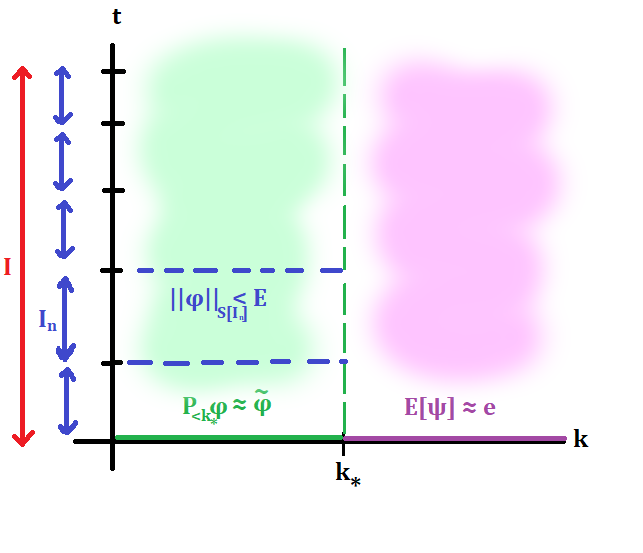
\includegraphics[scale = 0.7]{graphics/induction}
		\caption{Proposition \ref{prop:lowfreq} shows that the low frequencies are close. The high frequencies are controlled by the energy step via conservation of energy. The size of $\widetilde \phi$ in the $\sfS$-norm is large, so we divide into $O_{\widetilde \cF} (1)$-many sub-intervals on which the norm is comparable to the energy. We conclude the argument using perturbation theory on each sub-interval. 
		}
	\end{center}
\end{figure}

We first establish uniform energy bounds for $\psi$. As $\phi$ and $\widetilde\phi$ are wave maps, they have conserved energy $\cE[\phi] = \cE$ and $\cE[\widetilde \phi] \equiv \cE + e$ respectively. Thus, using Proposition \ref{prop:lowfreq}, one can conclude their difference has energy on the order $\cE[\psi] \lesssim e$. 

\begin{lemma}[Almost energy conservation]
	Let $\phi$ be a wave map with energy $\cE[\phi] = \cE + e$, and denote $\widetilde \phi$ the wave map with initial data $\widetilde \phi[0] = \Pi P_{\leq k_*} \phi[0]$ and energy $\cE[\widetilde \phi] = \cE$. If $\phi$ and $\widetilde \phi$ are defined on the time interval $J$, their difference $\psi := \phi - \widetilde \phi$ satisfies the almost conservation of energy
		\begin{equation}
			\cE[\psi(t)] \lesssim e\label{eq:psiconserve}
		\end{equation}
	for all $t \in J$. 
\end{lemma}

\begin{proof}
	Decomposing into high and low frequencies $\phi = P_{> k_*} \phi + P_{\leq k_*} \phi$ and viewing the energy as arising from the inner product on $\dot H^1 \times L^2$, we can write
		\[
			\cE[\phi] = \cE[P_{> k_*} \phi] + \cE[P_{\leq k_*} \phi] + 2 \langle P_{> k_*} \phi, P_{\leq k_*} \phi \rangle_{\dot H^1 \times L^2}.
		\]
	The Littlewood-Paley projections are non-negative operators, so the inner product on the right is non-negative. On the other hand, the estimate \eqref{lowfreq} from Proposition \ref{prop:lowfreq} states that the low frequency terms $\widetilde \phi$ and $P_{\leq k_*} \phi$ are close, so, in particular, the reverse triangle inequality implies
		\[
			\left|\cE[P_{\leq k_*} \phi] - \cE[\widetilde \phi]\right| + \left|\cE[\psi] - \cE[P_{> k_*} \phi]\right| \leq 100K_1 (\cF) \epsilon^{\delta_0}. 
		\]
	Collecting our results, we obtain
		\begin{align*}
			\cE[\psi]
				&\leq \cE[P_{> k_*} \phi] + 100 \epsilon^{\delta_0} K(\cF) \\
				&\leq \cE[\phi] - \cE[P_{\leq k_*} \phi] + 100\epsilon^{\delta_0} K(\cF)\\
				&\leq \cE[\phi] - \cE[\widetilde \phi] + 200 \epsilon^{\delta_0} K (\cF) \\
				&\leq e +  200 \epsilon^{\delta_0} K (\cF)
		\end{align*}	
	Making appropriate choices of $\epsilon$ and $\cF$ completes the proof. 	
\end{proof}

Next, we prove partial divisibility for the $\sfS$-norm. For functions with finite $L^p_t$-norm for $1 \leq p < \infty$, we can divide the interval into sub-intervals on which the $L^p_t$-norms are small. However, since the $\sfS$-norm contains $L^\infty_t$-norms, one cannot hope for divisibility into arbitrarily small norms, but one can divide into norms on the order of the energy. 


\begin{lemma}[Partial divisibility]
	Let $\widetilde \phi$ be a wave map on the interval $J$ with energy $\cE[\widetilde \phi] = \cE$ and space-time control $||\phi||_{\sfS[J]} = \widetilde \cF$. Then there exists a non-decreasing positive function $K_2 (\widetilde \cF) > 0$ of polynomial growth such that we can partition the time interval into $K_2 (\widetilde \cF)$-many sub-intervals $J = \bigsqcup J_k$ such that 
		\begin{equation}
			||\widetilde \phi||_{\sfS[J_k]} \lesssim \cE.\label{eq:divis}
		\end{equation}
\end{lemma}

\begin{proof}
	See \cite[Section 10.2]{SterbenzTataru2010}
\end{proof}

Finally, we can use the perturbation theory as in the previous section to obtain good estimates for the $\sfS$-norm of $\psi$ on each sub-interval. The coefficients $\widetilde \phi$ have size on the order of the energy, we can choose the energy step $e \ll 1$ sufficiently small, depending \textit{only} on energy, to close the continuity argument. 

\begin{lemma}[Perturbation theory for $\psi$]
	Let $\widetilde \phi$ be a wave map and $\psi$ a solution to the equation for the evolution of high frequencies
	\begin{equation}
		\Box \psi
			= - \bfS (\widetilde \phi) \partial^\alpha \widetilde \phi \partial_\alpha \widetilde \phi + \bfS (\widetilde \phi + \psi) \partial^\alpha( \widetilde \phi + \psi) \partial_\alpha (\widetilde \phi + \psi).
			 \label{eq:highwave}
	\end{equation}
	Suppose $\widetilde\phi$ has space-time norm controlled by the energy $\cE > 0$ on an interval $J$ as in \eqref{divis}, and $\psi$ has energy smaller than $e(\cE) \ll 1$ uniformly in time as in \eqref{psiconserve}, that is 
		\begin{align}
			||\widetilde \phi||_{\sfS[J]} 
				&\lesssim \cE \label{eq:lowphicontrol},\\
			\cE[\psi(t)] 
				&\lesssim e(\cE), \qquad \text{for $t \in J$}\label{eq:psicontrol}
		\end{align}
	then $\psi$ also admits the space-time control over the time interval $J$, 
	\begin{equation}
		||\psi||_{\sfS[J]} \leq 1. \label{eq:pert}
	\end{equation}
\end{lemma}

\begin{proof}
	Without loss of generality, suppose $J$ is centered at $t = 0$. Using the estimate \eqref{psicontrol} for $e (\cE) \ll 1$ and the energy estimate, there exists a small time interval $J_0 \subseteq J$ on which the conclusion of the lemma holds. We propagate this base case by making the bootstrap assumption
		\begin{equation}
			||\psi||_{\sfS[I]} \leq 2
		\label{eq:pertBA}
		\end{equation}
	for some sub-interval $I \subseteq J$, and aim to improve to \eqref{pert}. 
		\begin{equation}
			||\psi + \widetilde \phi||_{\sfS[I]} + ||\widetilde \phi||_{\sfS[I]} \lesssim_\cE 1. 
		\end{equation}
	Claim 
		\begin{equation}
			||\psi||_{\sfS_{\lambda c} [I]} \lesssim_\cE 1
		\end{equation}
	for $\lambda = e + \widetilde \epsilon^{\delta_0 \delta_1^2}$. The paradifferential version
		\begin{equation}
			\Box \psi_k + 2 \bfA^\alpha (\phi)_{< k - m} \partial_\alpha \psi_k = \text{perturbative}
		\end{equation}	
		{\color{red} ADD ALGEBRAIC DECOMPOSITION AND ESTIMATES FOR PERTURBATIVE TERMS}		
\end{proof}


\begin{proposition}[High frequency evolution]
	Let $\phi$ and $\widetilde \phi$ be defined as in Lemma \ref{prop:lowfreq}. There exists a function of energy $e(\cE)$ and a non-decreasing positive function $K_2 (\widetilde \cF) > 0$ of polynomial growth such that if $e \leq e(\cE)$ then
		\begin{equation}
			||\phi - \widetilde \phi||_{\sfS[J]} \leq K_2 (\widetilde \cF). 
		\end{equation}
\end{proposition}

\begin{proof}
	Triangle inequality
		\[  
			||\phi||_{\sfS[J]} \leq \sum_{k = 1}^{K_2 (\widetilde \cF)} ||\phi||_{\sfS[J_k]} \leq K_2 (\widetilde \cF). 
		\]
\end{proof}

\bibliographystyle{alpha}
\bibliography{external/biblio}

\end{document}
